\section{Background}

Before we can begin to answer the questions, we must select the materials used and calculate the reverberation times in the conference room and single office.


\subsection{Materials}

The design team has recommended using a double lightweight partition between the conference room and single office, together with the use of carpeted floors, plastered walls and a suspended ceiling inside the two rooms.
According to the assignment description, the suspended ceiling consists of mineral fibre tiles over a 1000~mm air space, and the partition is made up of two 12.5~mm plasterboard sheets on each side of a 100~mm or 120~mm cavity completely filled with mineral wool.

The remaining materials (for the walls, floors and windows) have been selected for a worst case scenario, i.e. these materials have the lowest absorption coefficients amongst their counterparts.
All materials used in the rooms are presented in Table~\ref{tbl:absorption} along with their absorption coefficients.
(Note that we are using absorption coefficients for a 100~mm cavity partition.)

It is likely that the thin carpet on concrete and 10~mm double glazed windows will be the cheapest among their counterparts, since they do not absorb sound as well.
It will be interesting to find out whether the cheapest and ``worst performing" materials in the proposed design solution will meet the intelligibility and privacy requirements of the conference room.
If they do not, one can then consider using more absorptive (and possibly more expensive) materials.


% Please add the following required packages to your document preamble:
% \usepackage{booktabs}
\begin{table}[htbp]
	\caption{Absorption coefficients of the materials used in the conference room and single office.}
	\label{tbl:absorption}
	\centering
	\begin{tabular}{@{}lrrrrrrr@{}}
		\toprule
		Frequency (Hz) & 63 & 125 & 250 & 500 & 1000 & 2000 & 4000 \\ \midrule
		Thin carpet on concrete & 0.01 & 0.01 & 0.02 & 0.05 & 0.15 & 0.30 & 0.40 \\
		Plaster on solid backing & 0.02 & 0.02 & 0.03 & 0.04 & 0.05 & 0.07 & 0.08 \\
		Plasterboard on 100 mm cavity with mineral wool & 0.12 & 0.30 & 0.12 & 0.08 & 0.06 & 0.06 & 0.05 \\
		Mineral fibre tile, 1000 mm airspace & 0.74 & 0.77 & 0.74 & 0.68 & 0.85 & 0.85 & 0.80 \\
		Double glazing, 10 mm gap & 0.07 & 0.10 & 0.07 & 0.05 & 0.03 & 0.02 & 0.02 \\ \bottomrule
	\end{tabular}
\end{table}


\subsubsection{Absorption coefficients}

The materials' absorption coefficients at 63~Hz had to be extrapolated.
This was done by identifying what types of sound absorbers the materials are and using their properties to estimate the materials' absorption coefficents at 63~Hz (see Figure~\ref{fig:absorbers}).


\begin{figure}[htbp]
	\centering
	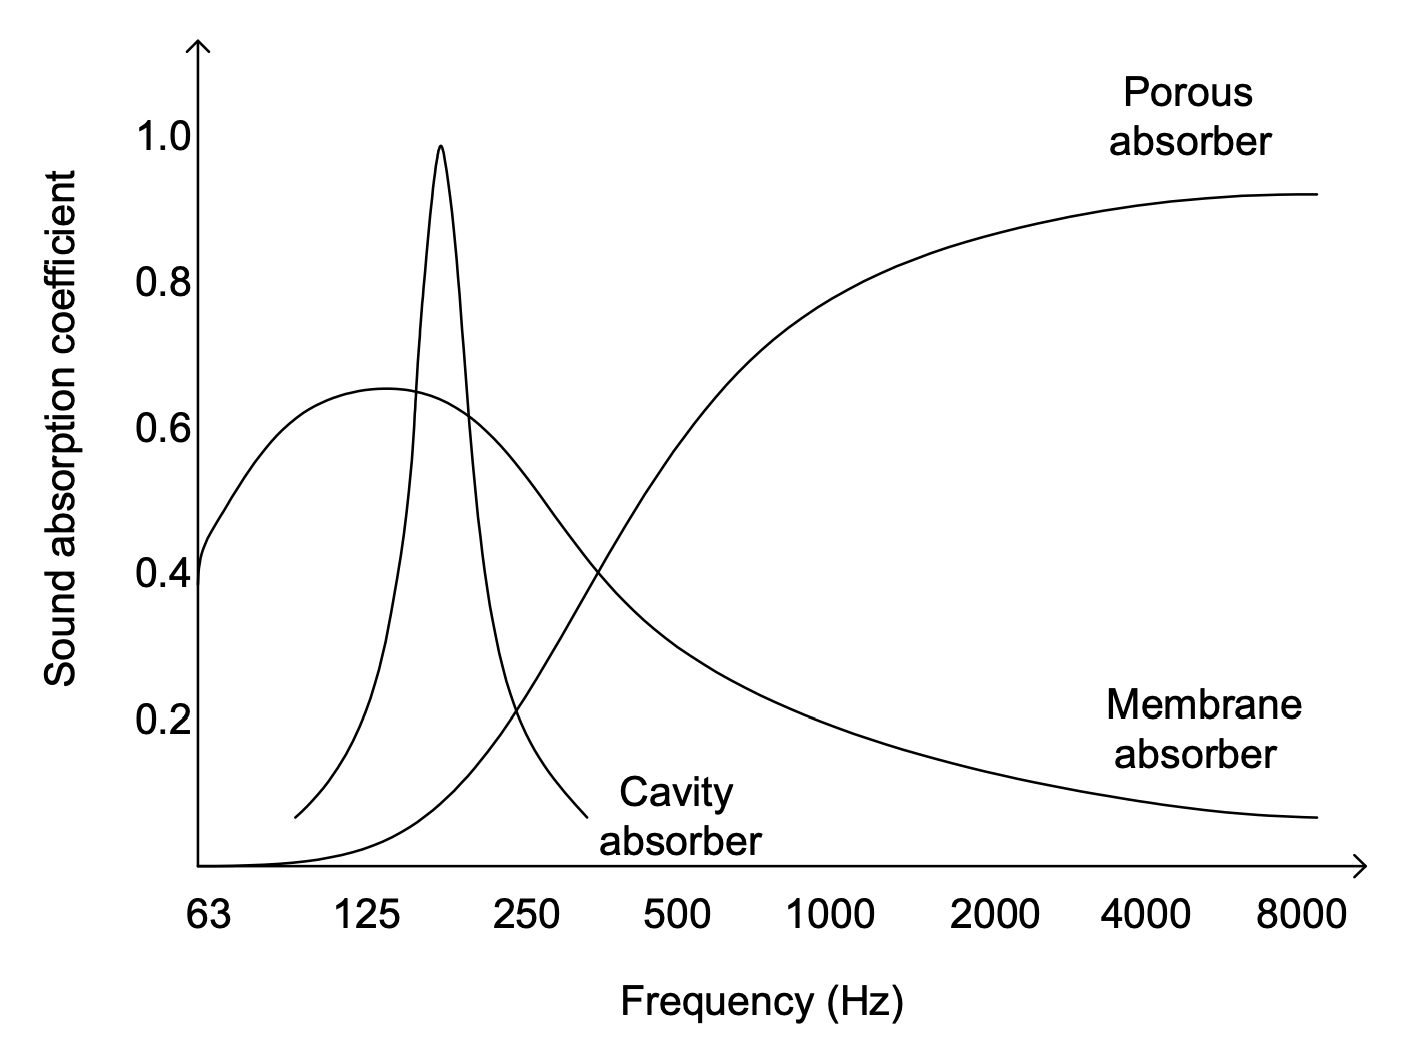
\includegraphics[width=.6\textwidth]{figures/Absorbers.png}
	\rule{.8\textwidth}{0.5pt} % use line???
	\caption{Absorption coefficients of sound absorbers \citep{Galbrun2018}.}
	\label{fig:absorbers}
\end{figure}


Carpet is a porous absorber, which absorbs very efficiently at high frequencies.
Its mid-frequency absorption properties can be improved by increasing its thickness.
Since absorption is almost constant between 63~Hz and 125~Hz, we have chosen the absorption coefficient at 63~Hz to be identical to that at 125~Hz (i.e. 0.01).

Double glazed windows are membrane absorbers, which absorb most effectively at frequencies below 500~Hz.
Changing the panel mass or depth of the air space can change the frequency of maximum absorption.
According to Figure~\ref{label}, the absorption coefficients at 63~Hz and 250~Hz are similar, hence we have chosen the absorption coefficient at 63~Hz to be identical to that at 250~Hz (i.e. 0.07).

The cavity-filled partition and mineral fibre suspended ceiling are both porous and membrane absorbers, hence they combine the absorption properties of the two absorber types.
Since the partition and suspended ceiling behave as membrane absorbers on the lower end of the frequency spectrum, we have chosen the absorption coefficients at 63~Hz to be identical to those at 250~Hz (i.e. respectively 0.12 and 0.74).

As for the plaster on solid backing, which is neither a porous nor membrane absorber, we assumed the absorption coefficient at 63~Hz to be identical to that at 125~Hz (i.e. 0.02) to match the subtle increase of absorption coefficients with frequency.

The absorption coefficients of the materials used in the rooms are presented in Table~\ref{tbl:absorption} and Figure~\ref{fig:absorption_coefs}.


\begin{figure}[htbp]
	\centering
	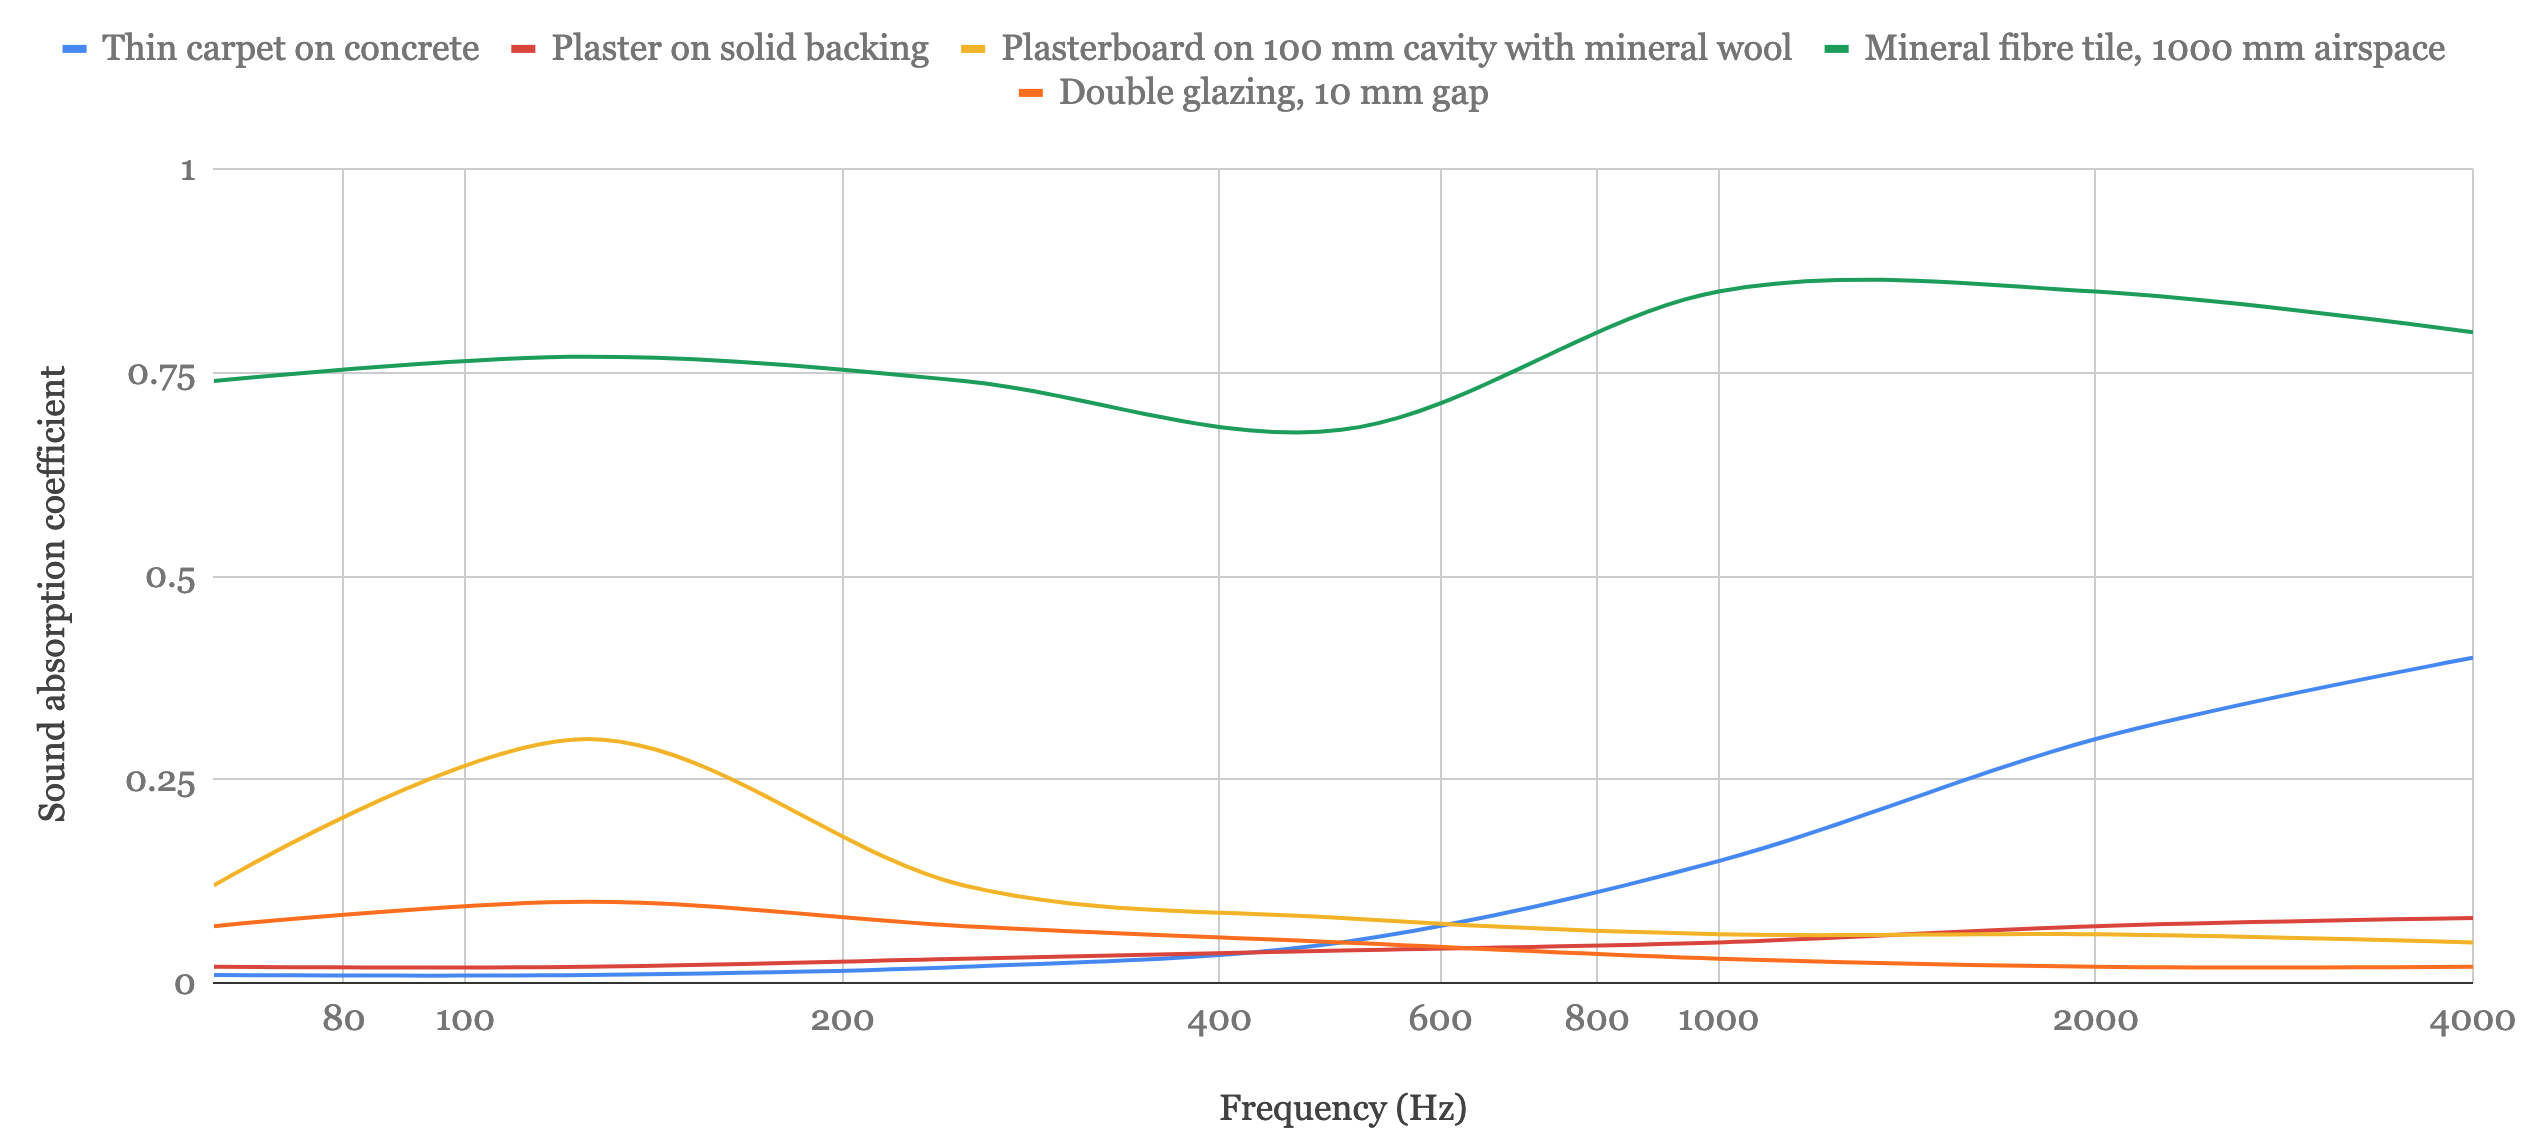
\includegraphics[width=\textwidth]{figures/Materials_absorption.png}
	\rule{\textwidth}{0.5pt} % use line???
	\caption{Absorption coefficients of the materials used in the conference room and single office.}
	\label{fig:absorption_coefs}
\end{figure}




\subsection{Reverberation times}

The reverberation times of either or both the conference room and single office are needed to calculate the sound pressure levels (SPLs) and standardised level differences (D\textsubscript{nT}) in Questions 1, 3 and 4.
Equation~\ref{eq:reverb} gives Sabine's formula for calculating the reverberation time, T (s), in a room of volume V (m\textsuperscript{3}) and total absorption $\Sigma$A (m\textsuperscript{2}).
The absorption of a surface, A, is the product of the surface area, S (m\textsuperscript{2}), and the surface's absorption coefficient, $\alpha$.

    \begin{equation}\label{eq:reverb}
		T = \frac{0.161 V}{\Sigma A} = \frac{0.161 V}{\Sigma S \alpha}
	\end{equation}

The dimensions and volumes of the conference room and single office are presented in Table~\ref{tbl:room_dims}.
This information and the absorption coefficients of the surfaces allow us to calculate the reverberation times of the rooms.
Table~\ref{tbl:reverb_conf_example} provides the details of the calculations at 63~Hz in the conference room.
Tables~\ref{tbl:reverb_conf} and \ref{tbl:reverb_office} respectively present the calculations at all frequencies in the conference room and single office.

Figure \ref{fig:reverb_times} presents the reverberation times of the rooms in graphical form.
The curves are similar because the materials and constructions in the rooms are the same.
The single office has reverberation times that are between 0.01~s and 0.03~s smaller than those of the conference room.
This is because the single office has a smaller volume than the conference room.
The arithmetic averages of the reverberation times in the conference room and single office are respectively 0.41~s and 0.40~s.
Considering that the typical reverberation time of rooms used for speech is between 0.5~s and 1.0~s, these results are a bit low.
This might be perceived as uncomfortable by the occupants, especially when they and the furnishings will further add absorption and shorten the reverberation times in the rooms.

% Please add the following required packages to your document preamble:
% \usepackage{booktabs}
\begin{table}[htbp]
	\caption{Dimensions of the conference room, single office and partition wall.}
	\label{tbl:room_dims}
	\centering
	\begin{tabular}{@{}lrrrrr@{}}
		\toprule
		Dimensions & \multicolumn{1}{l}{Width (m)} & \multicolumn{1}{l}{Depth (m)} & \multicolumn{1}{l}{Height* (m)} & \multicolumn{1}{l}{Area (m\textsuperscript{2})} & \multicolumn{1}{l}{Volume* (m\textsuperscript{3})} \\ \midrule
		Conference room\textsubscript{(1)} & 8 & 4 & 2.5 & - & 80 \\
		Single office\textsubscript{(2)} & 5 & 4 & 2.5 & - & 50 \\
		Partition wall & - & 4 & 2.5 & 10 & - \\ \bottomrule
		\multicolumn{6}{l}{*\textit{Under the suspended ceiling}} \\
		\multicolumn{6}{l}{\textsubscript{(1)} \textit{The subscript ``1" refers to the conference room throughout the rest of the report.}} \\
		\multicolumn{6}{l}{\textsubscript{(2)} \textit{The subscript ``2" refers to the single office throughout the rest of the report.}}
	\end{tabular}
\end{table}

% Please add the following required packages to your document preamble:
% \usepackage{booktabs}
\begin{sidewaystable}[htbp]
	\caption{Details of the reverberation time calculations at 63~Hz in the conference room.}
	\label{tbl:reverb_conf_example}
	\centering
	\begin{tabular}{@{}lrrrr@{}}
		\toprule
		Frequency (Hz) & \multicolumn{1}{l}{} & \multicolumn{1}{c}{} & \multicolumn{2}{c}{63} \\ \midrule
		Surface & $S$ (m\textsuperscript{2}) & \multicolumn{1}{l}{} & \multicolumn{1}{c}{$\alpha$} & $S \alpha = A$ (m\textsuperscript{2}) \\
		Floor & $8 \times 4 = 32$ &  & 0.01 & $32 \times 0.01 = 0.32$ \\
		Ceiling & $8 \times 4 = 32$ &  & 0.74 & $32 \times 0.74 = 23.68$ \\
		Windows & 8 &  & 0.07 & $8 \times 0.07 = 0.56$ \\
		Partition wall & $4 \times 2.5 = 10$ &  & 0.12 & $10 \times 0.12 = 1.20$ \\
		Plastered walls & $2 \times 2.5 (8 + 4) - S_{windows} - S_{partition} = 2 \times 2.5 (8 + 4) - 8 - 10 = 42$ &  & 0.02 & $42 \times 0.02 = 0.84$ \\ \midrule
		Total absorption (m\textsuperscript{2}) &  &  &  & $\Sigma S \alpha = \Sigma A = 26.60$ \\
		Reverberation time (s) &  &  &  & $T = \frac{0.161 V_{1}}{\Sigma A} = \frac{0.161 \times 80}{26.60} = 0.48$ \\ \bottomrule
	\end{tabular}
\end{sidewaystable}

% Please add the following required packages to your document preamble:
% \usepackage{booktabs}
\begin{sidewaystable}[htbp]
	\caption{Calculation of the reverberation times in the conference room.}
	\label{tbl:reverb_conf}
	\centering
	\begin{tabular}{@{}m{3cm}rrrrrrrrrrrrrrrrrrrrrr@{}}
		\toprule
		Frequency (Hz) & \multicolumn{1}{l}{} & \multicolumn{1}{c}{} & \multicolumn{2}{c}{63} & \multicolumn{1}{c}{} & \multicolumn{2}{c}{125} & \multicolumn{1}{c}{} & \multicolumn{2}{c}{250} & \multicolumn{1}{c}{} & \multicolumn{2}{c}{500} & \multicolumn{1}{c}{} & \multicolumn{2}{c}{1000} & \multicolumn{1}{c}{} & \multicolumn{2}{c}{2000} & \multicolumn{1}{c}{} & \multicolumn{2}{c}{4000} \\ \midrule
		Surface & \multicolumn{1}{l}{S (m\textsuperscript{2})} & \multicolumn{1}{l}{} & \multicolumn{1}{c}{$\alpha$} & \multicolumn{1}{c}{A} & \multicolumn{1}{c}{} & \multicolumn{1}{c}{$\alpha$} & \multicolumn{1}{c}{A} & \multicolumn{1}{c}{} & \multicolumn{1}{c}{$\alpha$} & \multicolumn{1}{c}{A} & \multicolumn{1}{c}{} & \multicolumn{1}{c}{$\alpha$} & \multicolumn{1}{c}{A} & \multicolumn{1}{c}{} & \multicolumn{1}{c}{$\alpha$} & \multicolumn{1}{c}{A} & \multicolumn{1}{c}{} & \multicolumn{1}{c}{$\alpha$} & \multicolumn{1}{c}{A} & \multicolumn{1}{c}{} & \multicolumn{1}{c}{$\alpha$} & \multicolumn{1}{c}{A} \\
		Floor & 32 &  & 0.01 & 0.32 &  & 0.01 & 0.32 &  & 0.02 & 0.64 &  & 0.05 & 1.60 &  & 0.15 & 4.80 &  & 0.30 & 9.60 &  & 0.40 & 12.80 \\
		Ceiling & 32 &  & 0.74 & 23.68 &  & 0.77 & 24.64 &  & 0.74 & 23.68 &  & 0.68 & 21.76 &  & 0.85 & 27.20 &  & 0.85 & 27.20 &  & 0.80 & 25.60 \\
		Windows & 8 &  & 0.07 & 0.56 &  & 0.10 & 0.80 &  & 0.07 & 0.56 &  & 0.05 & 0.40 &  & 0.03 & 0.24 &  & 0.02 & 0.16 &  & 0.02 & 0.16 \\
		Partition wall & 10 &  & 0.12 & 1.20 &  & 0.30 & 3.00 &  & 0.12 & 1.20 &  & 0.08 & 0.80 &  & 0.06 & 0.60 &  & 0.06 & 0.60 &  & 0.05 & 0.50 \\
		Plastered walls & 42 &  & 0.02 & 0.84 &  & 0.02 & 0.84 &  & 0.03 & 1.26 &  & 0.04 & 1.68 &  & 0.05 & 2.10 &  & 0.07 & 2.94 &  & 0.08 & 3.36 \\ \midrule
		Total absorption $\Sigma S \alpha = \Sigma A$ (m\textsuperscript{2}) &  &  &  & 26.60 &  &  & 29.60 &  &  & 27.34 &  &  & 26.24 &  &  & 34.94 &  &  & 40.50 &  &  & 42.42 \\
		Reverberation time T (s) &  &  &  & 0.48 &  &  & 0.44 &  &  & 0.47 &  &  & 0.49 &  &  & 0.37 &  &  & 0.32 &  &  & 0.30 \\ \bottomrule
	\end{tabular}
\end{sidewaystable}

% Please add the following required packages to your document preamble:
% \usepackage{booktabs}
\begin{sidewaystable}[htbp]
	\caption{Calculation of the reverberation times in the single office.}
	\label{tbl:reverb_office}
	\centering
	\begin{tabular}{@{}b{3cm}rrrrrrrrrrrrrrrrrrrrrr@{}}
		\toprule
		Frequency (Hz) & \multicolumn{1}{l}{} & \multicolumn{1}{l}{} & \multicolumn{2}{c}{63} & \multicolumn{1}{c}{} & \multicolumn{2}{c}{125} & \multicolumn{1}{c}{} & \multicolumn{2}{c}{250} & \multicolumn{1}{c}{} & \multicolumn{2}{c}{500} & \multicolumn{1}{c}{} & \multicolumn{2}{c}{1000} & \multicolumn{1}{c}{} & \multicolumn{2}{c}{2000} & \multicolumn{1}{c}{} & \multicolumn{2}{c}{4000} \\ \midrule
		Surface & S (m\textsuperscript{2}) & \multicolumn{1}{l}{} & \multicolumn{1}{c}{$\alpha$} & \multicolumn{1}{c}{A} & \multicolumn{1}{c}{} & \multicolumn{1}{c}{$\alpha$} & \multicolumn{1}{c}{A} & \multicolumn{1}{c}{} & \multicolumn{1}{c}{$\alpha$} & \multicolumn{1}{c}{A} & \multicolumn{1}{c}{} & \multicolumn{1}{c}{$\alpha$} & \multicolumn{1}{c}{A} & \multicolumn{1}{c}{} & \multicolumn{1}{c}{$\alpha$} & \multicolumn{1}{c}{A} & \multicolumn{1}{c}{} & \multicolumn{1}{c}{$\alpha$} & \multicolumn{1}{c}{A} & \multicolumn{1}{c}{} & \multicolumn{1}{c}{$\alpha$} & \multicolumn{1}{c}{A} \\
		Floor & 20 &  & 0.01 & 0.20 &  & 0.01 & 0.20 &  & 0.02 & 0.40 &  & 0.05 & 1.00 &  & 0.15 & 3.00 &  & 0.30 & 6.00 &  & 0.40 & 8.00 \\
		Ceiling & 20 &  & 0.74 & 14.80 &  & 0.77 & 15.40 &  & 0.74 & 14.80 &  & 0.68 & 13.60 &  & 0.85 & 17.00 &  & 0.85 & 17.00 &  & 0.80 & 16.00 \\
		Windows & 5 &  & 0.07 & 0.35 &  & 0.10 & 0.50 &  & 0.07 & 0.35 &  & 0.05 & 0.25 &  & 0.03 & 0.15 &  & 0.02 & 0.10 &  & 0.02 & 0.10 \\
		Partition wall & 10 &  & 0.12 & 1.20 &  & 0.30 & 3.00 &  & 0.12 & 1.20 &  & 0.08 & 0.80 &  & 0.06 & 0.60 &  & 0.06 & 0.60 &  & 0.05 & 0.50 \\
		Plastered walls & 30 &  & 0.02 & 0.60 &  & 0.02 & 0.60 &  & 0.03 & 0.90 &  & 0.04 & 1.20 &  & 0.05 & 1.50 &  & 0.07 & 2.10 &  & 0.08 & 2.40 \\ \midrule
		Total absorption $\Sigma S \alpha = \Sigma A$ (m\textsuperscript{2}) &  &  &  & 17.15 &  &  & 19.70 &  &  & 17.65 &  &  & 16.85 &  &  & 22.25 &  &  & 25.80 &  &  & 27.00 \\
		Reverberation time T (s) &  &  &  & 0.47 &  &  & 0.41 &  &  & 0.46 &  &  & 0.48 &  &  & 0.36 &  &  & 0.31 &  &  & 0.30 \\ \bottomrule
	\end{tabular}
\end{sidewaystable}

\begin{figure}[htbp]
	\centering
	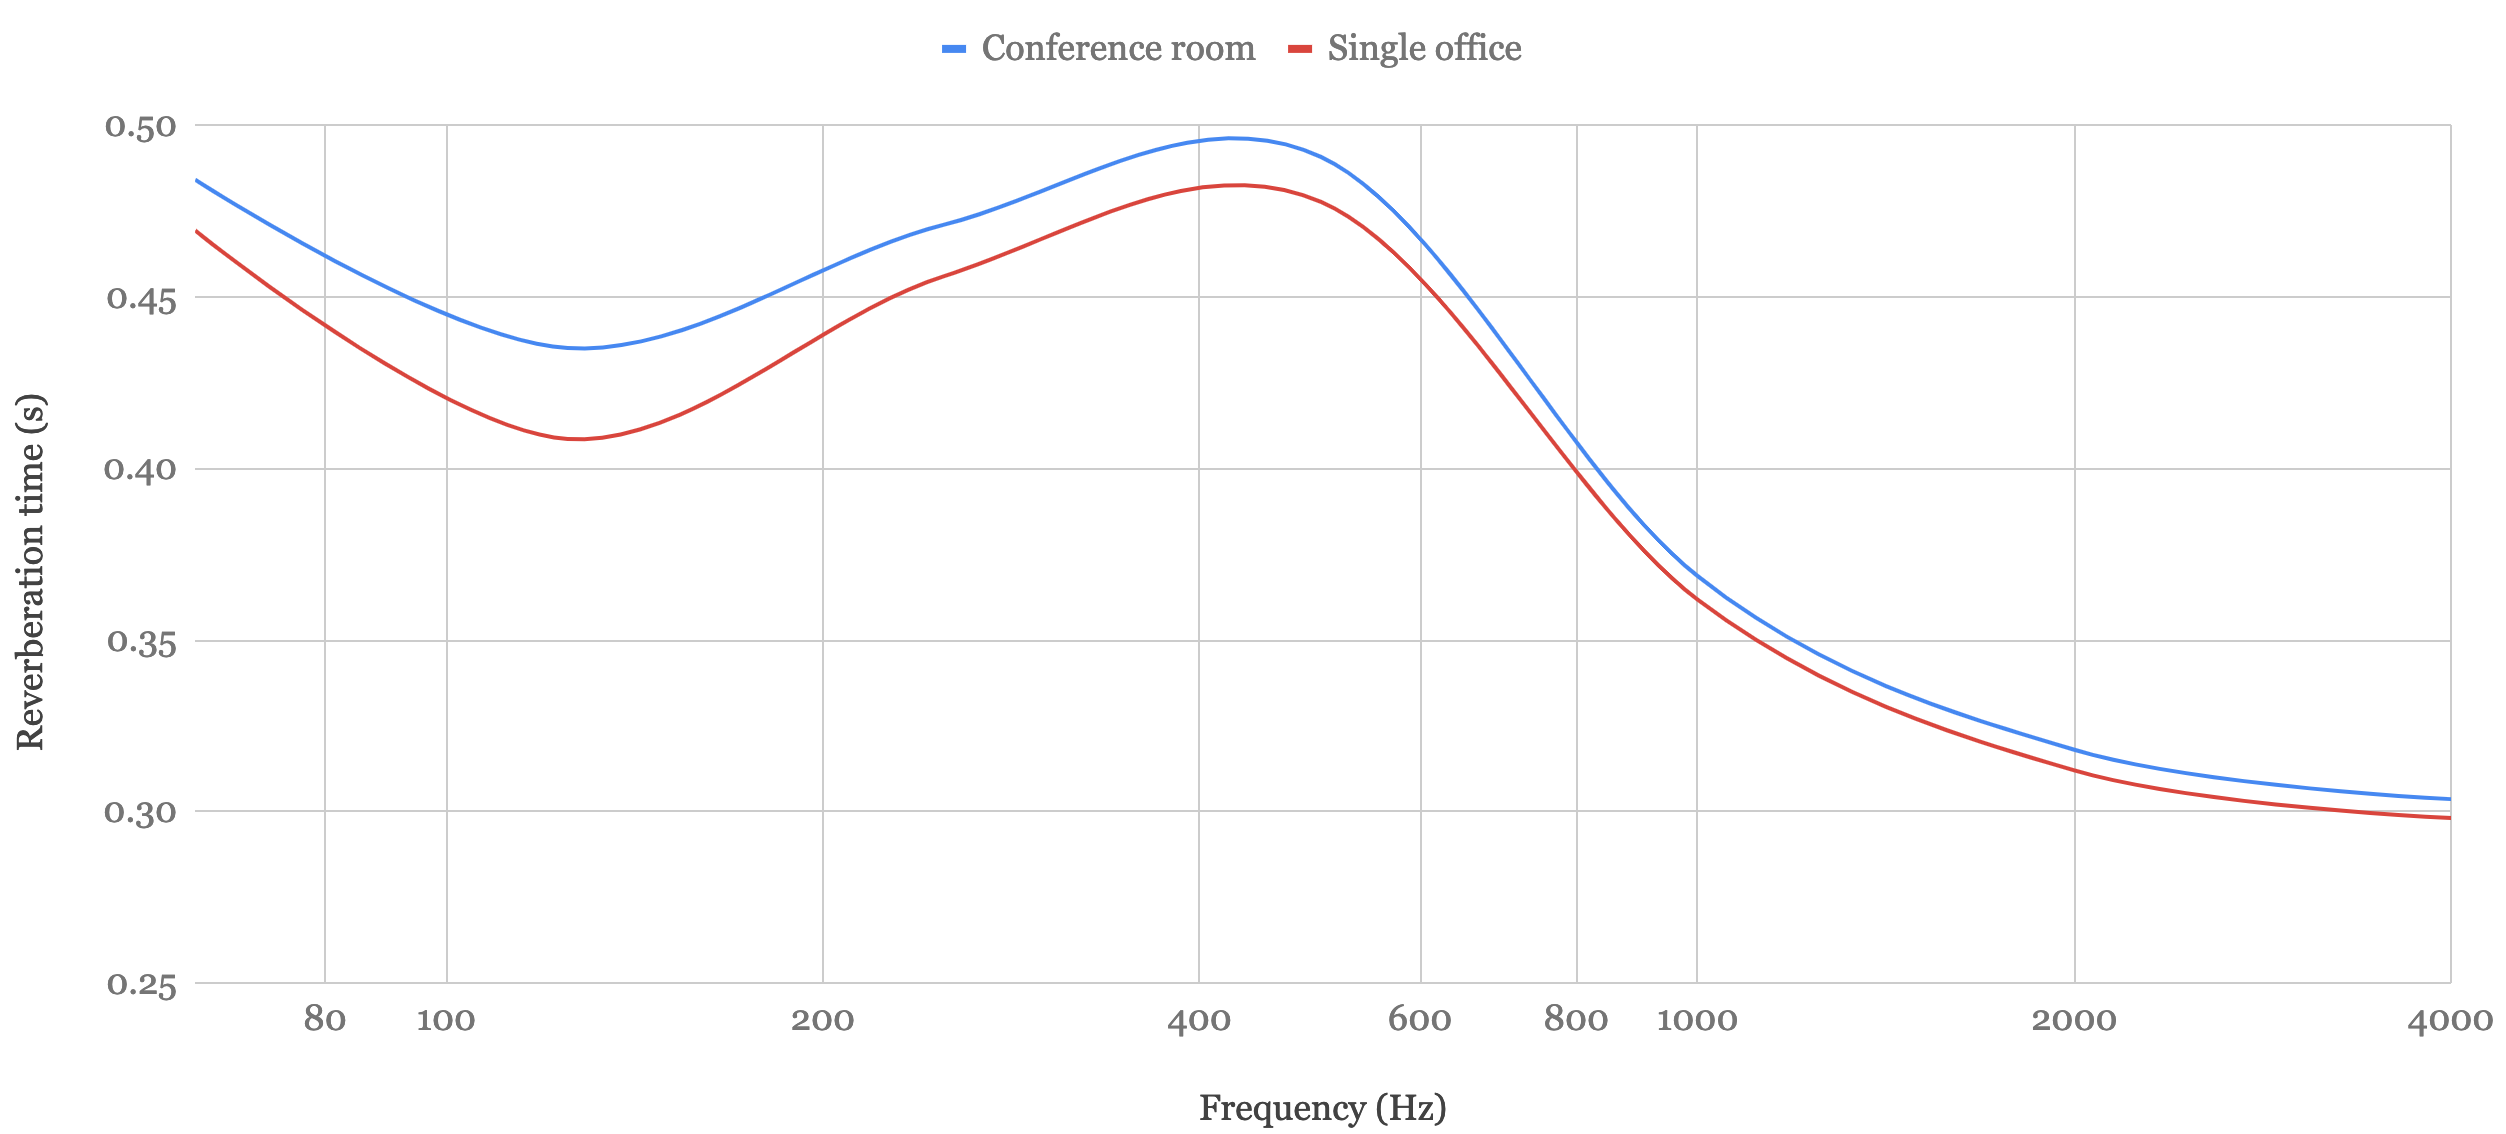
\includegraphics[width=\textwidth]{figures/Reverb_times.png}
	\rule{\textwidth}{0.5pt} % use line???
	\caption{Reverberation times in the conference room and single office.}
	\label{fig:reverb_times}
\end{figure}